\chapter{Grafik}

Beberapa grafik yang representatif. Lengkapnya terdapat pada link Google Drive pada lampiran sebelumnya.

\begin{figure}[h]
    %\centering
    \centerline{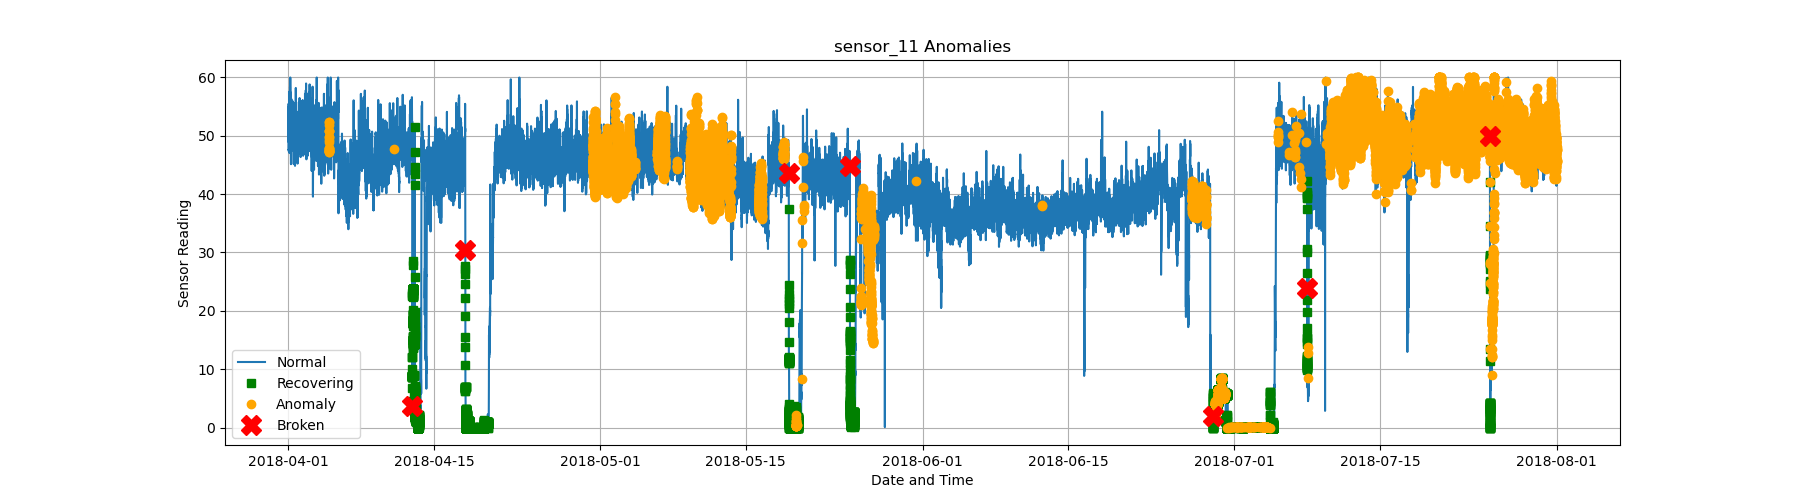
\includegraphics[width=1.4\textwidth]{resources/Acuan/IQR_sensor_11.png}}
    \caption{Hasil prediksi anomali model IQR} \label{IQR11}
\end{figure}
\begin{figure}[h]
    %\centering
    \centerline{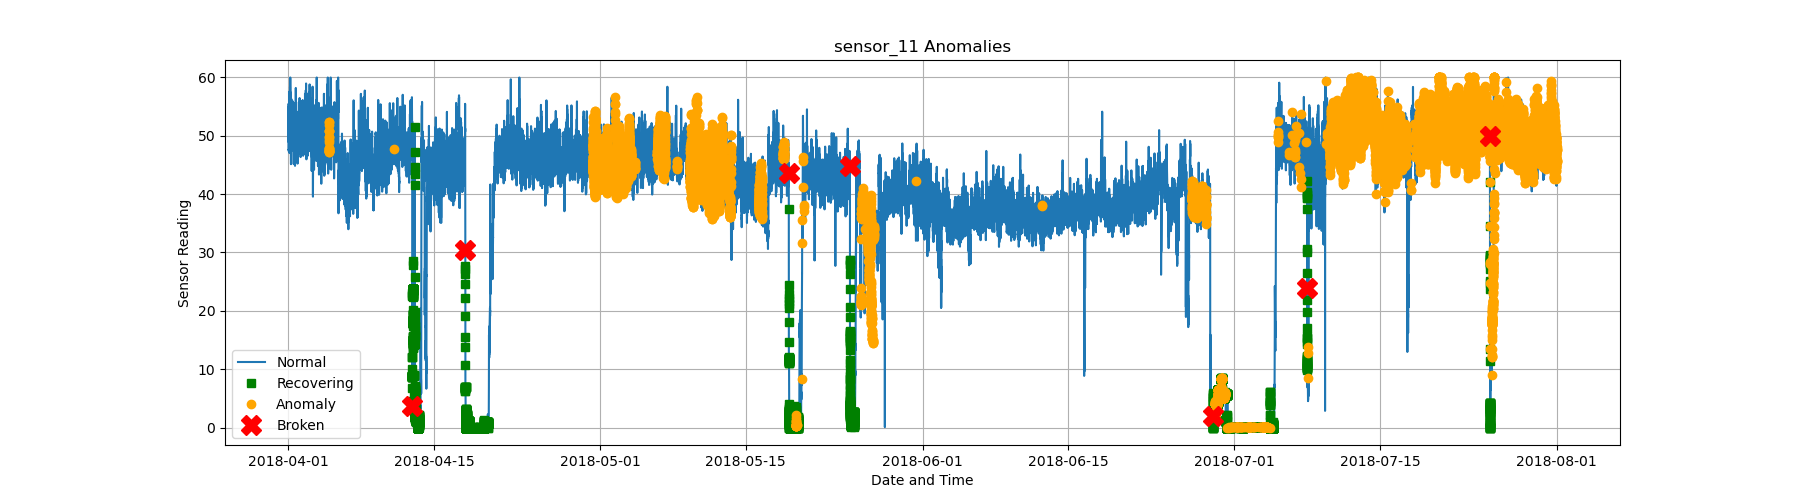
\includegraphics[width=1.4\textwidth]{resources/Acuan/KMeans_sensor_11.png}}
    \caption{Hasil prediksi anomali model K-Means Clustering} \label{KM11}
\end{figure}
\begin{figure}[h]
    %\centering
    \centerline{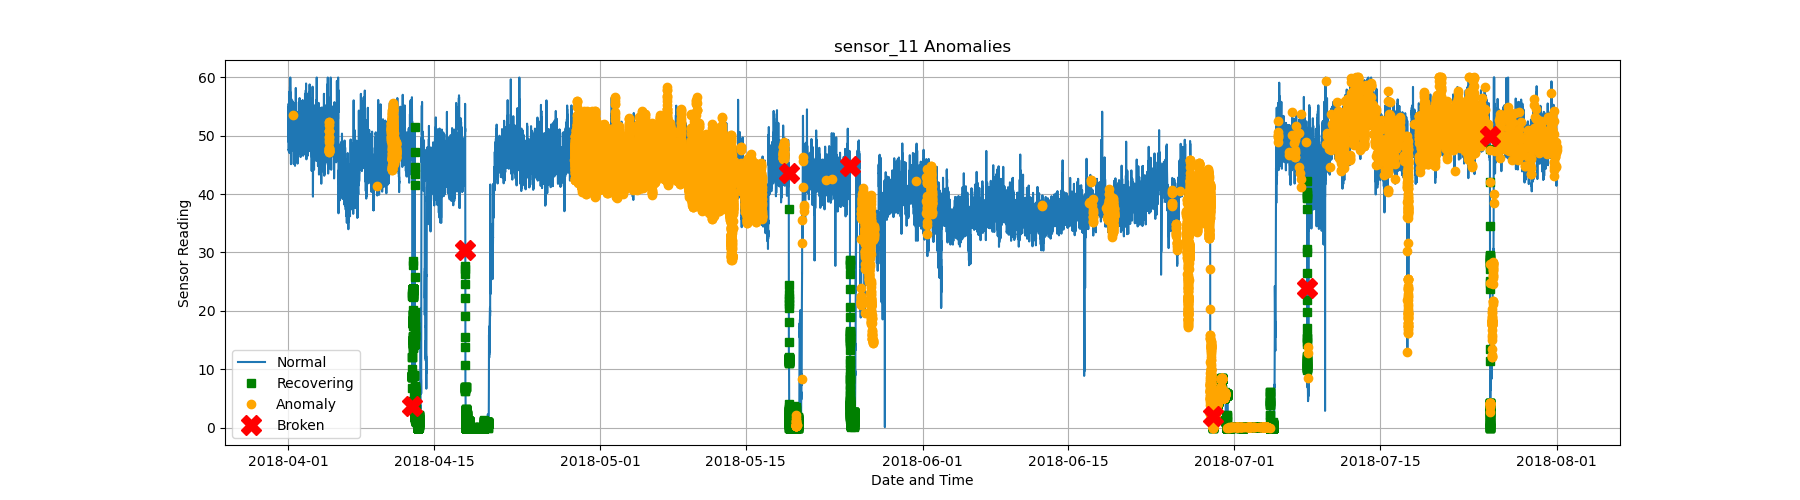
\includegraphics[width=1.4\textwidth]{resources/Acuan/IsoFor_sensor_11.png}}
    \caption{Hasil prediksi anomali model Isolation Forest} \label{IF11}
\end{figure}
\begin{figure}[h]
    %\centering
    \centerline{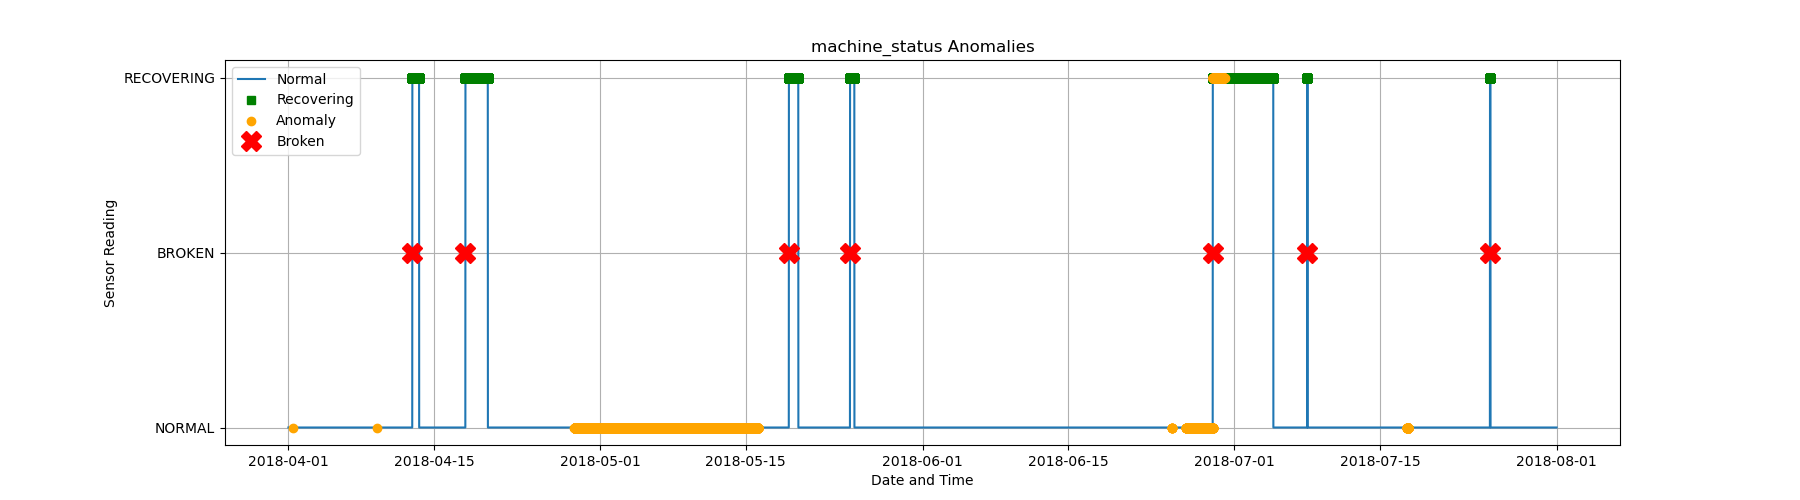
\includegraphics[width=1.4\textwidth]{resources/Acuan/IQR_machine_status.png}}
    \caption{Anomali model IQR dan status mesin} \label{IQRms}
\end{figure}
\begin{figure}[h]
    %\centering
    \centerline{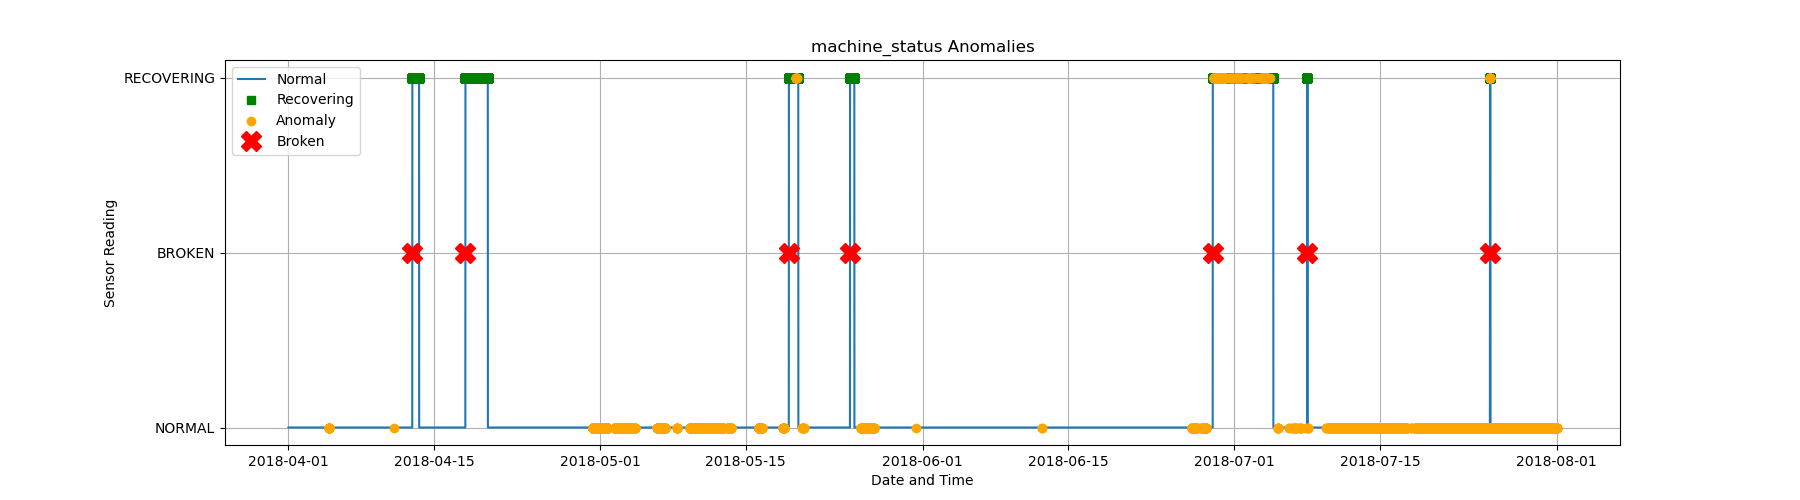
\includegraphics[width=1.4\textwidth]{resources/Acuan/KMeans_machine_status.png}}
    \caption{Anomali model K-Means Clustering dan status mesin} \label{KMms}
\end{figure}
\begin{figure}[h]
    %\centering
    \centerline{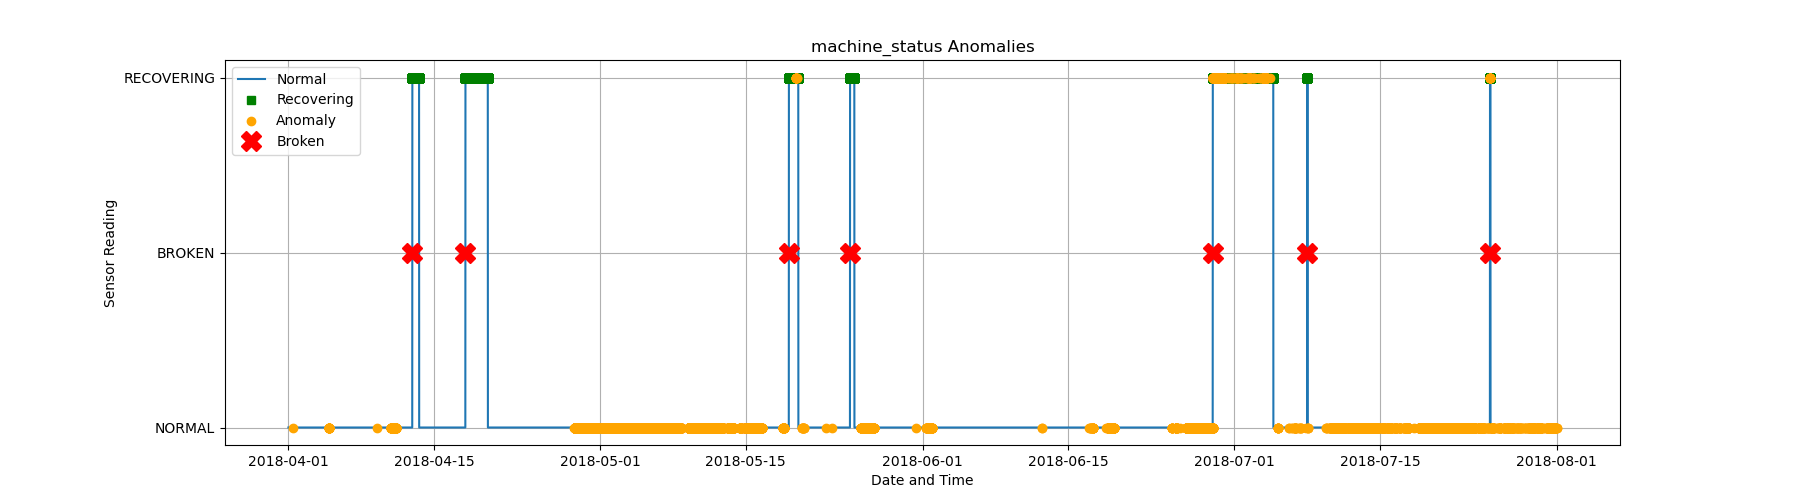
\includegraphics[width=1.4\textwidth]{resources/Acuan/IsoFor_machine_status.png}}
    \caption{Anomali model Isolation Forest dan status mesin} \label{IFms}
\end{figure}
\begin{figure}[h]
    %\centering
    \centerline{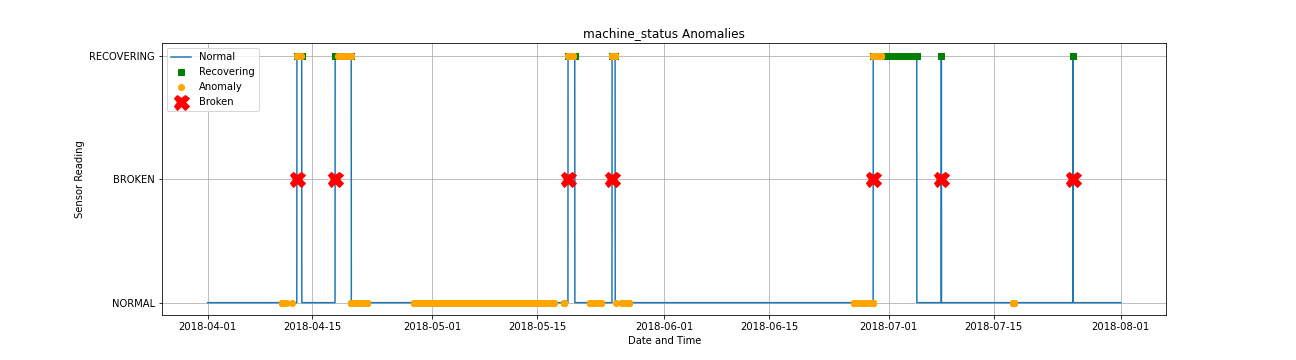
\includegraphics[width=1.4\textwidth]{resources/Bayes/Bayes_machine_status.png}}
    \caption{Anomali model Bayesian dan status mesin} \label{Bms}
\end{figure}
\begin{figure}[h]
    %\centering
    \centerline{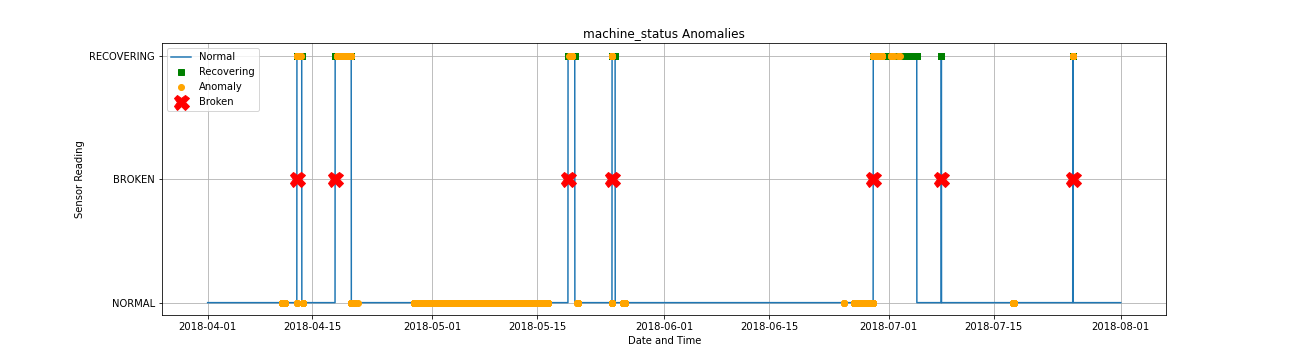
\includegraphics[width=1.4\textwidth]{resources/LSTM/LSTM_noPCA_machine_status.png}}
    \caption{Anomali model LSTM tanpa PCA dan status mesin} \label{nPms}
\end{figure}
\begin{figure}[h]
    %\centering
    \centerline{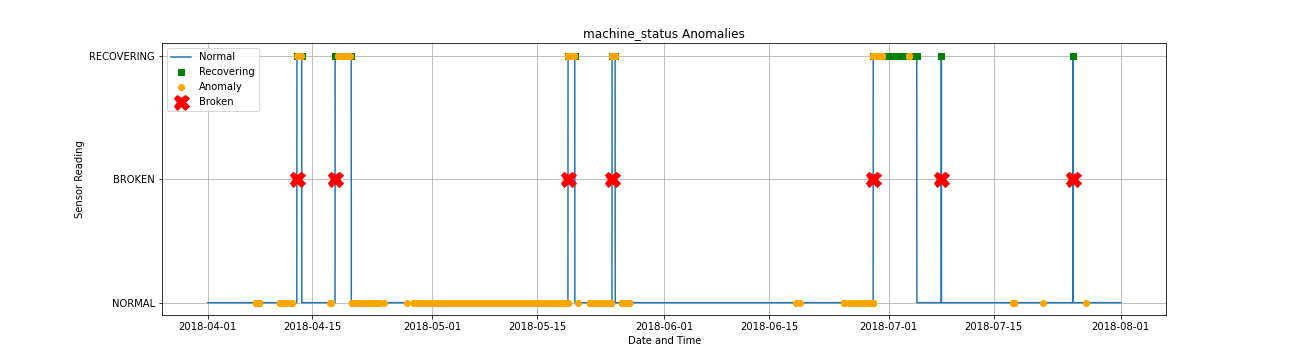
\includegraphics[width=1.4\textwidth]{resources/LSTM/LSTM_PCA_machine_status.png}}
    \caption{Anomali model LSTM dengan PCA dan status mesin} \label{wPms}
\end{figure}